% Editable native annotations around unchanged verified IDE photographs.
\par
\begin{figure}[htbp]
\centering
\newsavebox{\MARScrctableregistersBox}
\sbox{\MARScrctableregistersBox}{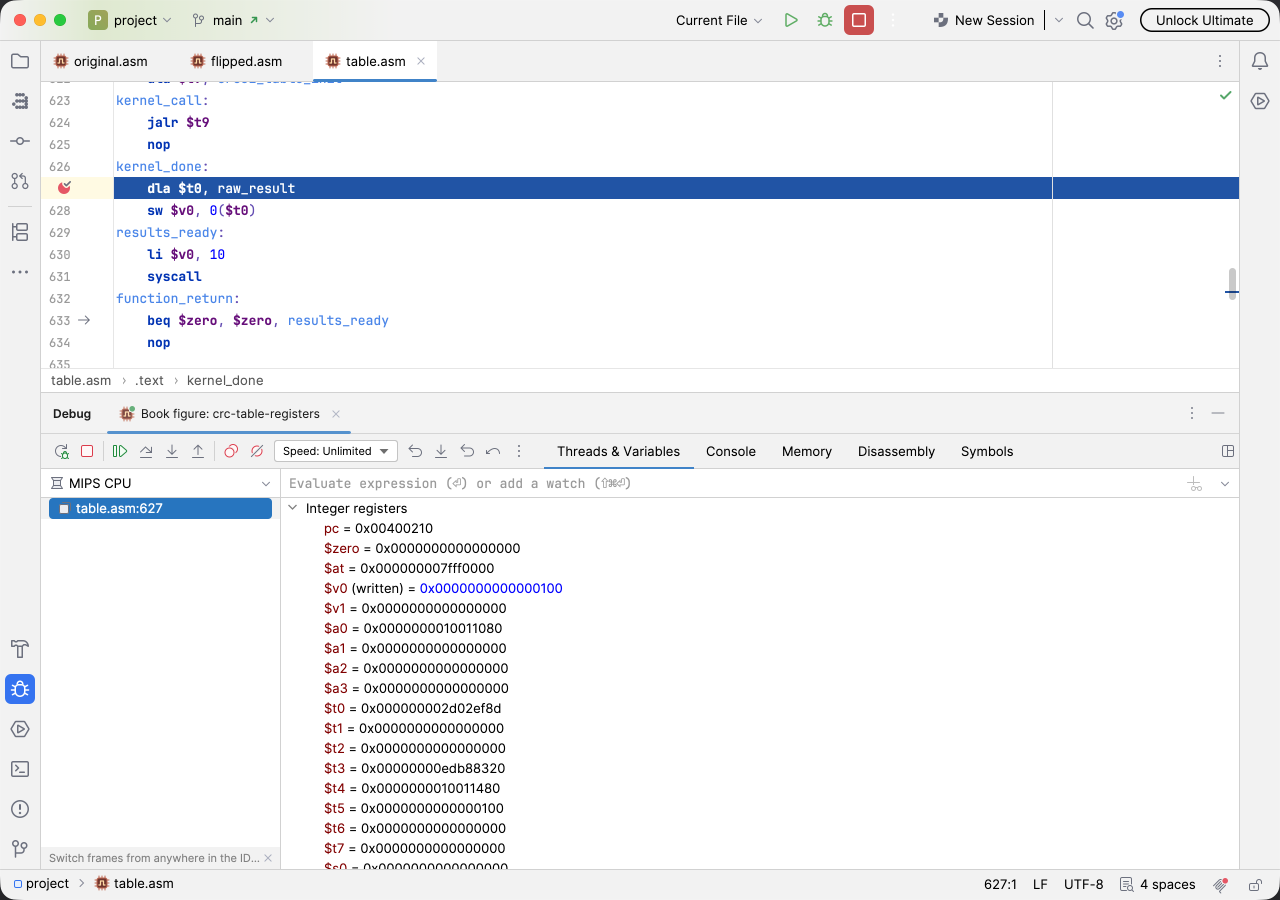
\includegraphics[artifact]{packages/024-crc32/captures/f02/registers.png}}
\newsavebox{\MARScrctablecursorBox}
\sbox{\MARScrctablecursorBox}{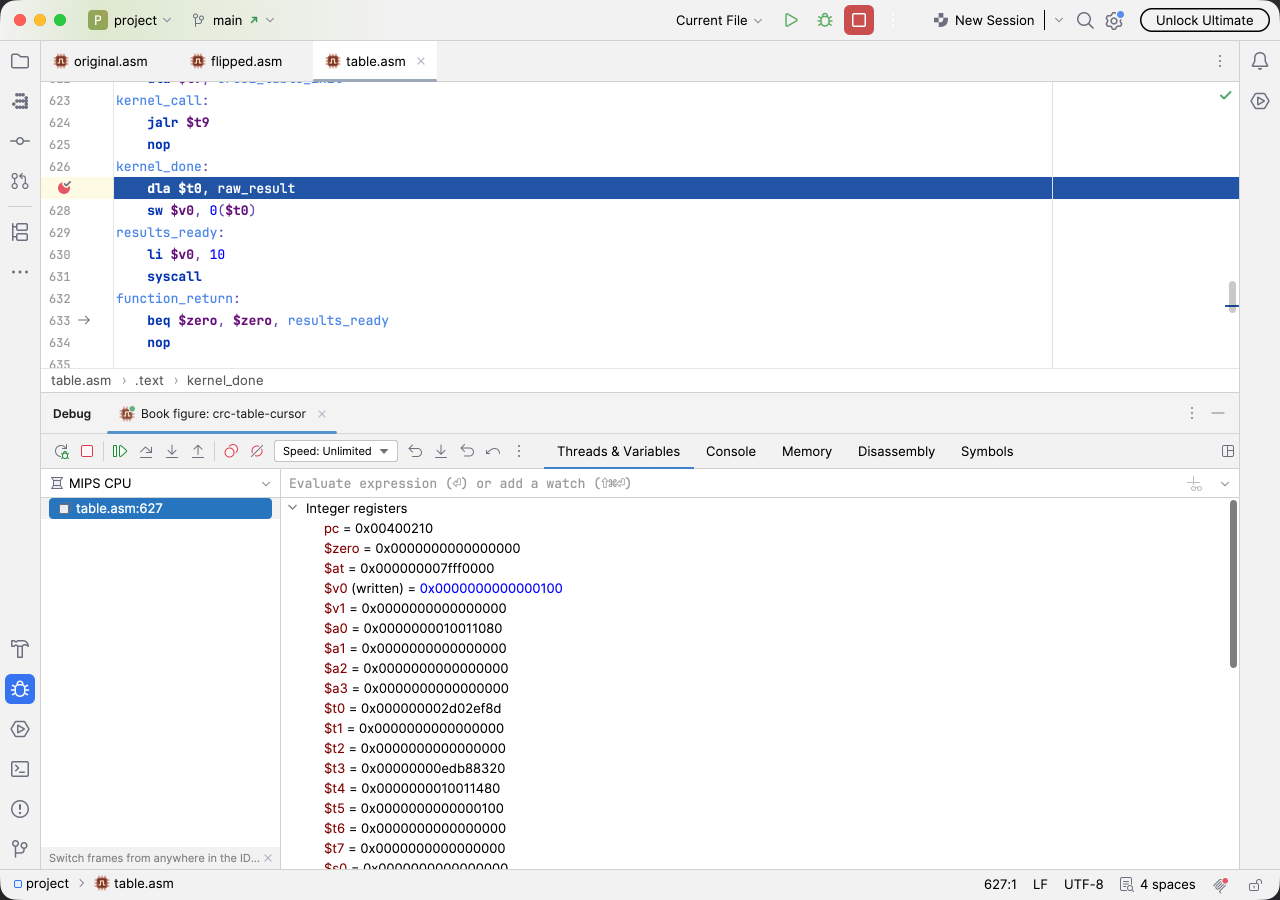
\includegraphics[artifact]{packages/024-crc32/captures/f02/cursor.png}}
\newsavebox{\MARScrctablezeroBox}
\sbox{\MARScrctablezeroBox}{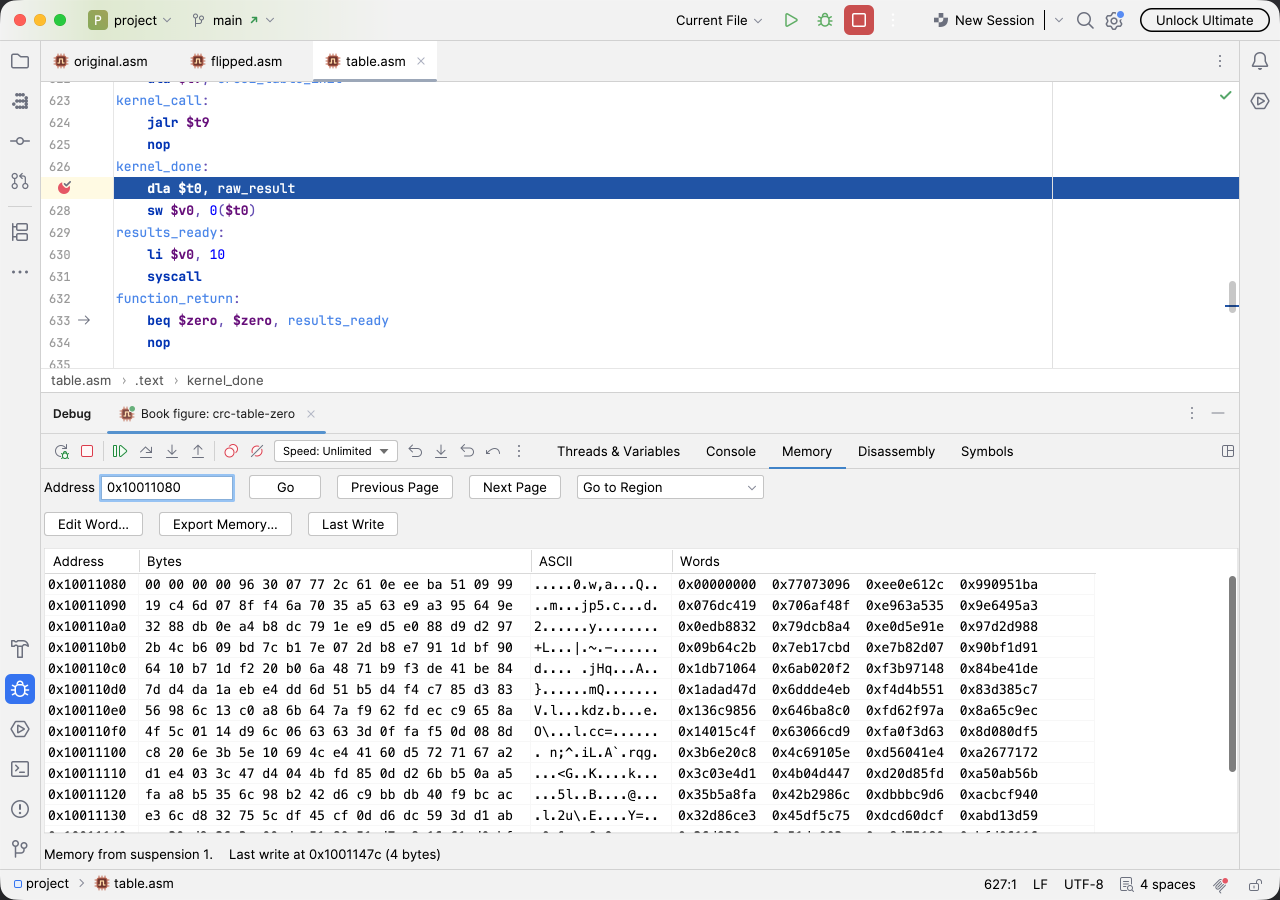
\includegraphics[artifact]{packages/024-crc32/captures/f02/zero.png}}
\newsavebox{\MARScrctablemiddleBox}
\sbox{\MARScrctablemiddleBox}{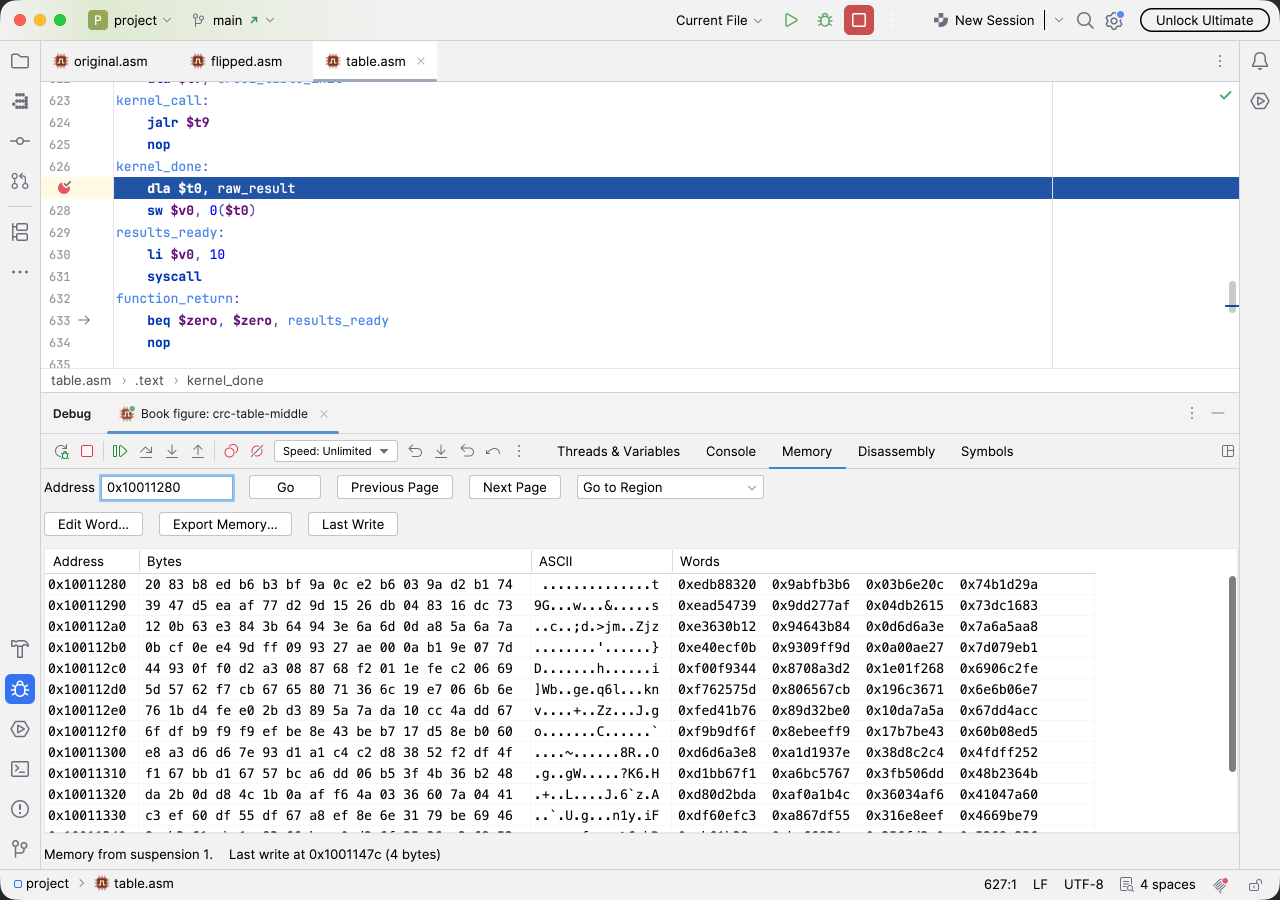
\includegraphics[artifact]{packages/024-crc32/captures/f02/middle.png}}
\newsavebox{\MARScrctabletailBox}
\sbox{\MARScrctabletailBox}{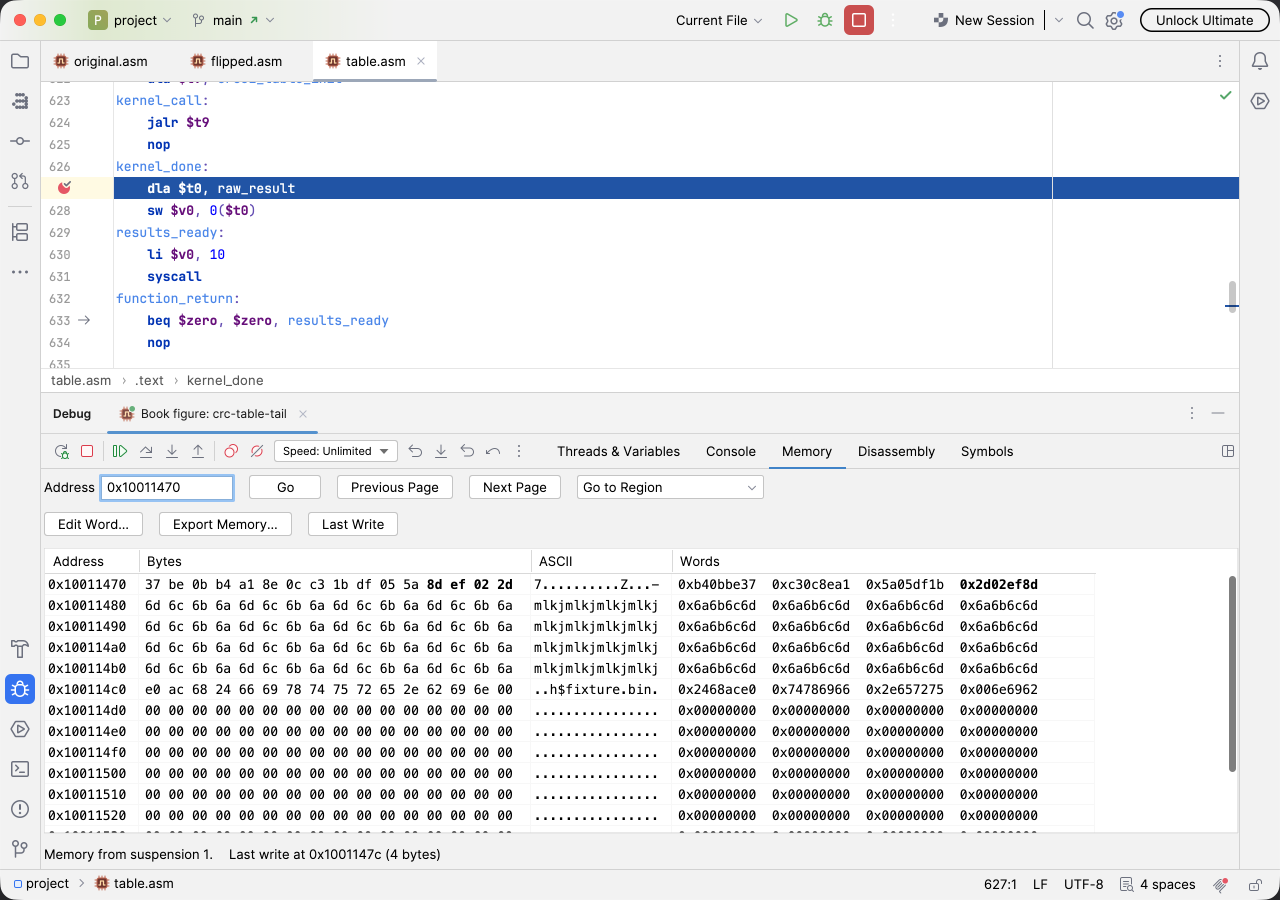
\includegraphics[artifact]{packages/024-crc32/captures/f02/tail.png}}
\newsavebox{\MARScrctableguardBox}
\sbox{\MARScrctableguardBox}{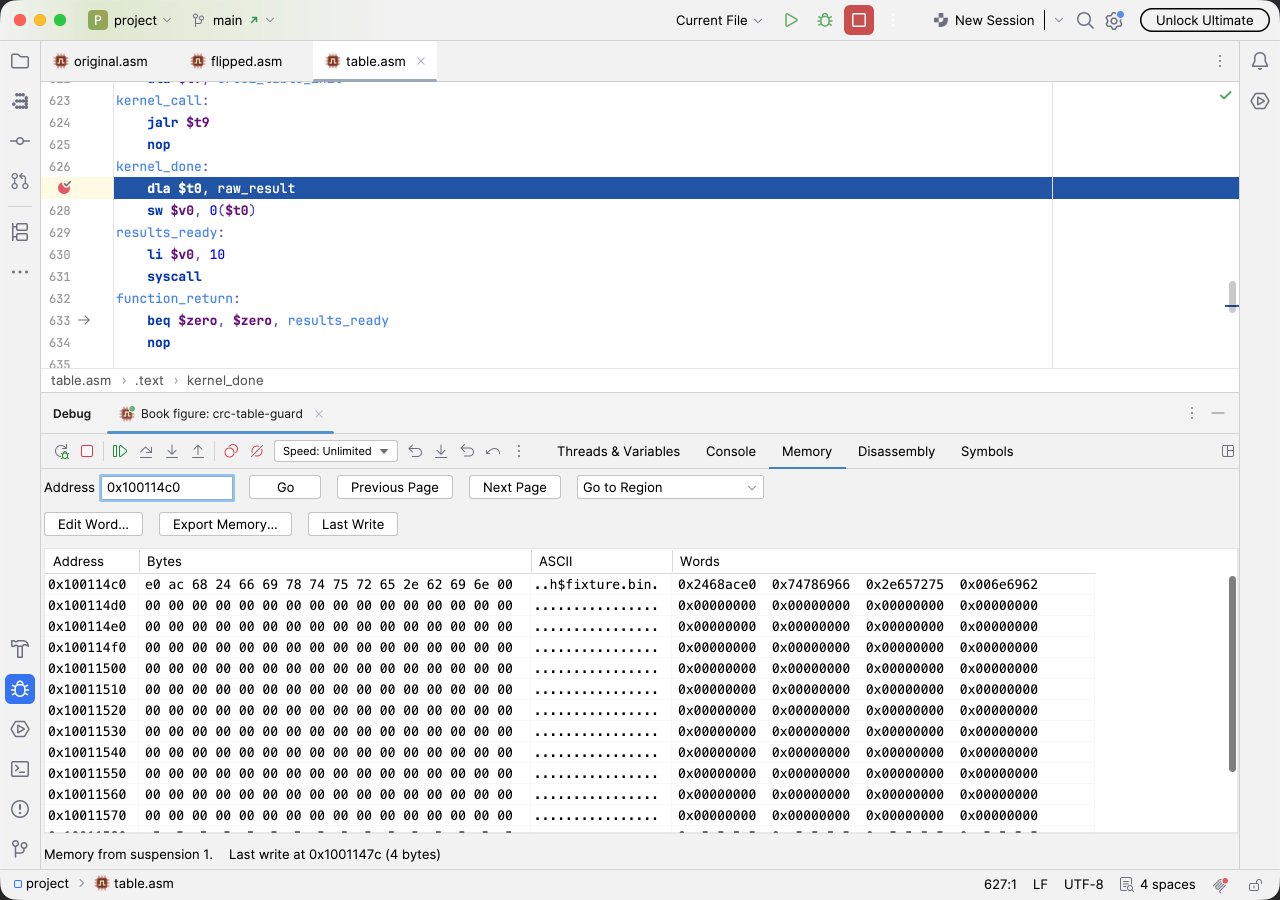
\includegraphics[artifact]{packages/024-crc32/captures/f02/guard.png}}
\edef\MARScrctablesourceLeft{\the\dimexpr0.036718750\wd\MARScrctableregistersBox\relax}
\edef\MARScrctablesourceBottom{\the\dimexpr0.774444444\ht\MARScrctableregistersBox\relax}
\edef\MARScrctablesourceRight{\the\dimexpr0.713281250\wd\MARScrctableregistersBox\relax}
\edef\MARScrctablesourceTop{\the\dimexpr0.170000000\ht\MARScrctableregistersBox\relax}
\edef\MARScrctablereturnsLeft{\the\dimexpr0.246093750\wd\MARScrctableregistersBox\relax}
\edef\MARScrctablereturnsBottom{\the\dimexpr0.334444444\ht\MARScrctableregistersBox\relax}
\edef\MARScrctablereturnsRight{\the\dimexpr0.553906250\wd\MARScrctableregistersBox\relax}
\edef\MARScrctablereturnsTop{\the\dimexpr0.640000000\ht\MARScrctableregistersBox\relax}
\edef\MARScrctablecursorLeft{\the\dimexpr0.246093750\wd\MARScrctablecursorBox\relax}
\edef\MARScrctablecursorBottom{\the\dimexpr0.090000000\ht\MARScrctablecursorBox\relax}
\edef\MARScrctablecursorRight{\the\dimexpr0.553906250\wd\MARScrctablecursorBox\relax}
\edef\MARScrctablecursorTop{\the\dimexpr0.862222222\ht\MARScrctablecursorBox\relax}
\edef\MARScrctablezeroLeft{\the\dimexpr0.034375000\wd\MARScrctablezeroBox\relax}
\edef\MARScrctablezeroBottom{\the\dimexpr0.334444444\ht\MARScrctablezeroBox\relax}
\edef\MARScrctablezeroRight{\the\dimexpr0.584375000\wd\MARScrctablezeroBox\relax}
\edef\MARScrctablezeroTop{\the\dimexpr0.608888889\ht\MARScrctablezeroBox\relax}
\edef\MARScrctablemiddleLeft{\the\dimexpr0.034375000\wd\MARScrctablemiddleBox\relax}
\edef\MARScrctablemiddleBottom{\the\dimexpr0.334444444\ht\MARScrctablemiddleBox\relax}
\edef\MARScrctablemiddleRight{\the\dimexpr0.584375000\wd\MARScrctablemiddleBox\relax}
\edef\MARScrctablemiddleTop{\the\dimexpr0.608888889\ht\MARScrctablemiddleBox\relax}
\edef\MARScrctabletailLeft{\the\dimexpr0.034375000\wd\MARScrctabletailBox\relax}
\edef\MARScrctabletailBottom{\the\dimexpr0.311111111\ht\MARScrctabletailBox\relax}
\edef\MARScrctabletailRight{\the\dimexpr0.584375000\wd\MARScrctabletailBox\relax}
\edef\MARScrctabletailTop{\the\dimexpr0.608888889\ht\MARScrctabletailBox\relax}
\edef\MARScrctableguardLeft{\the\dimexpr0.034375000\wd\MARScrctableguardBox\relax}
\edef\MARScrctableguardBottom{\the\dimexpr0.334444444\ht\MARScrctableguardBox\relax}
\edef\MARScrctableguardRight{\the\dimexpr0.584375000\wd\MARScrctableguardBox\relax}
\edef\MARScrctableguardTop{\the\dimexpr0.608888889\ht\MARScrctableguardBox\relax}
\begin{tikzpicture}[alt={Seven annotated details at kernel_done show return 256, cursor at the byte after 256 words and counter 256. Table entries zero, 128 and 255 are zero, edb88320 and 2d02ef8d. The sentinel suffix begins at logical entry 256 and the separate physical guard remains 2468ace0.}]
\node[anchor=north west,inner sep=0,font=\small\bfseries] (source-title) at (6mm,0) {Next instruction at this boundary};
\node[anchor=north west,inner sep=0] (source) at ([yshift=-1mm]source-title.south west) {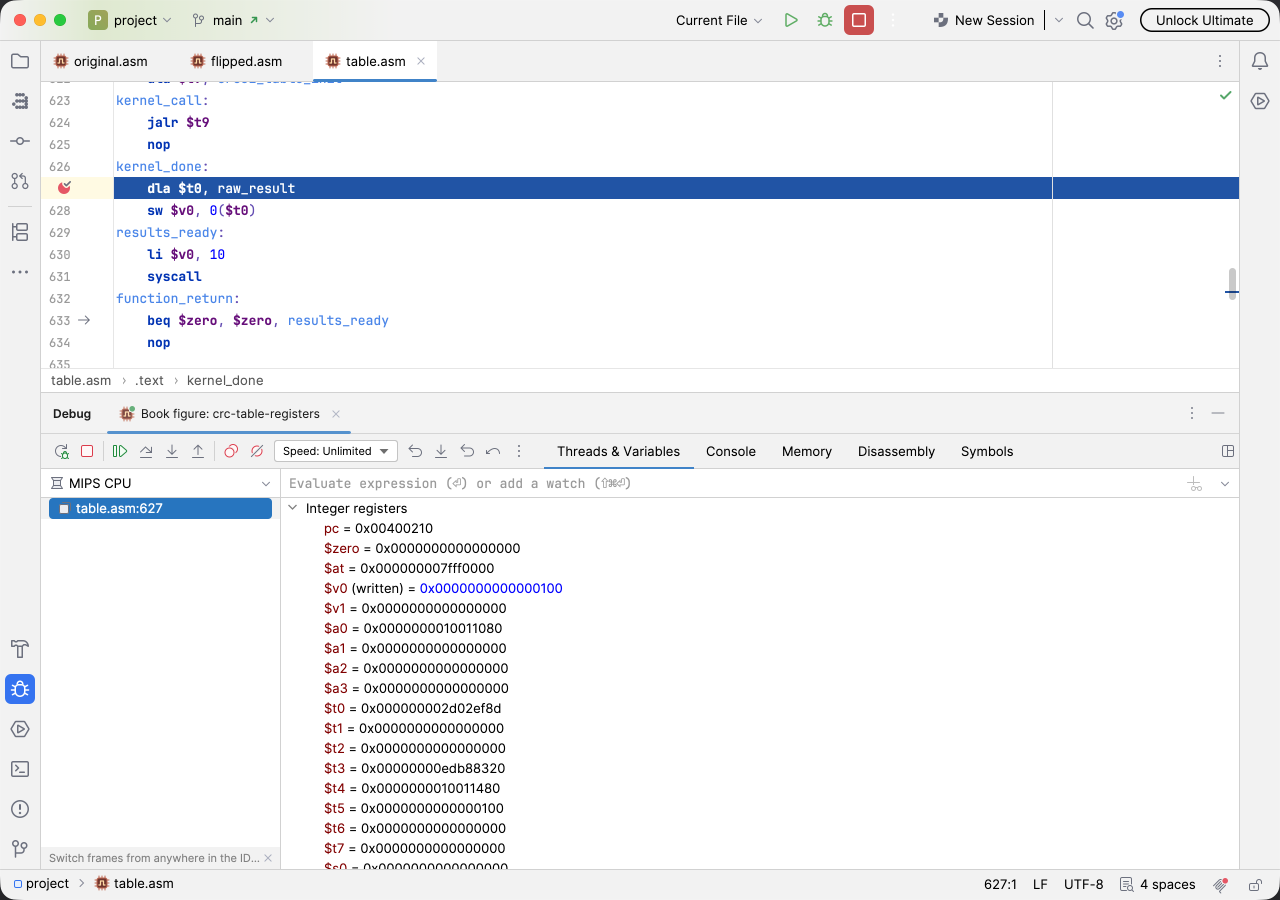
\includegraphics[width=0.54\linewidth,artifact,trim={\MARScrctablesourceLeft{} \MARScrctablesourceBottom{} \MARScrctablesourceRight{} \MARScrctablesourceTop{}},clip]{packages/024-crc32/captures/f02/registers.png}};
\begin{scope}[shift={(source.south west)},x={($(source.south east)-(source.south west)$)},y={($(source.north west)-(source.south west)$)}]
\draw[black,line width=0.7pt] (0.215625000,0.080000000) rectangle (0.775000000,0.520000000);
\node[draw=black,fill=white,circle,inner sep=1.5pt,font=\footnotesize] at ($(0.215625000,0.520000000)+(-3mm,0)$) {1};
\end{scope}
\node[anchor=north west,inner sep=0,font=\small\bfseries] (returns-title) at (0.58\linewidth,0 |- source-title.north) {Returned entry count};
\node[anchor=north west,inner sep=0] (returns) at ([yshift=-1mm]returns-title.south west) {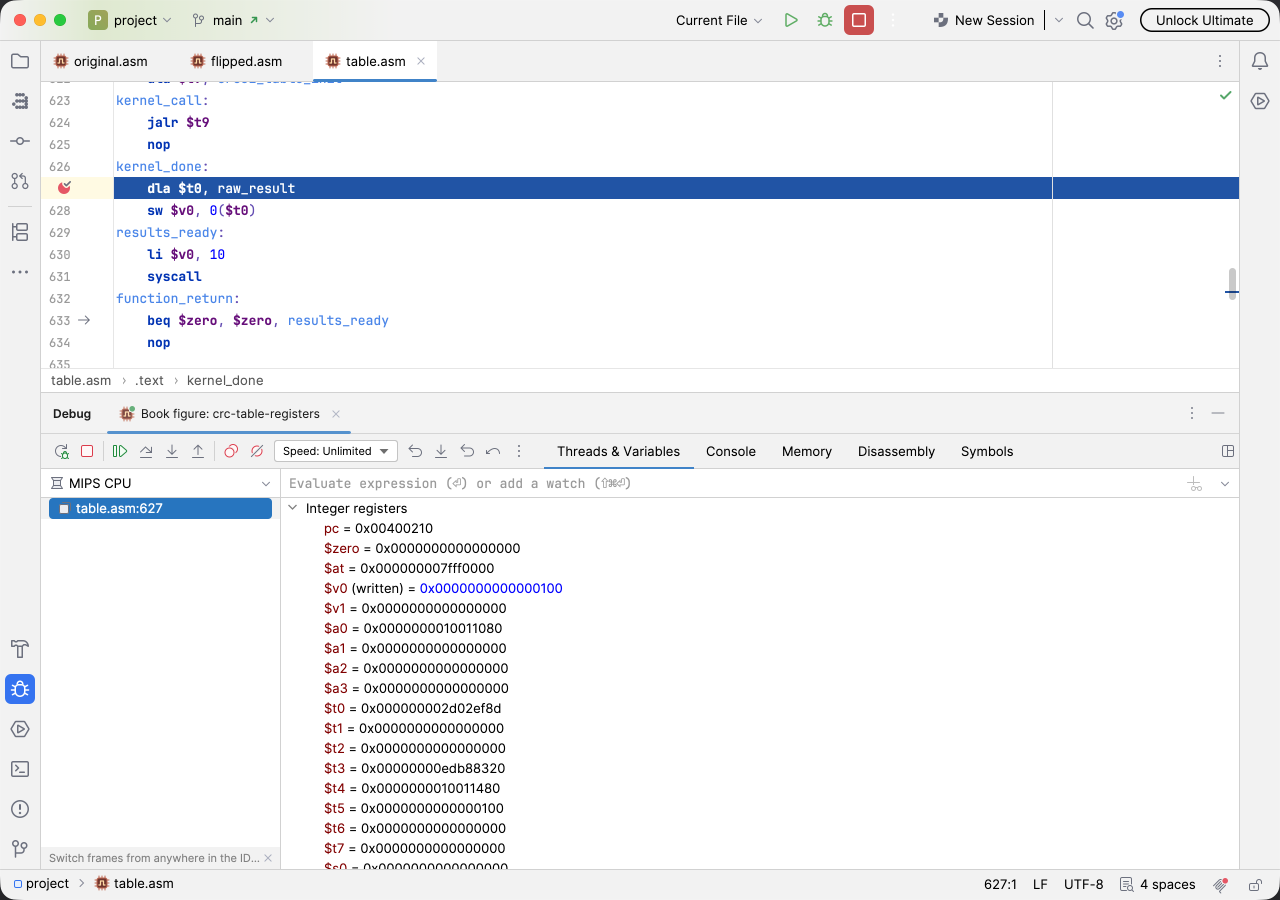
\includegraphics[width=0.42\linewidth,artifact,trim={\MARScrctablereturnsLeft{} \MARScrctablereturnsBottom{} \MARScrctablereturnsRight{} \MARScrctablereturnsTop{}},clip]{packages/024-crc32/captures/f02/registers.png}};
\begin{scope}[shift={(returns.south west)},x={($(returns.south east)-(returns.south west)$)},y={($(returns.north west)-(returns.south west)$)}]
\draw[black,line width=0.7pt] (0.023437500,0.043478261) rectangle (0.972656250,0.913043478);
\node[draw=black,fill=white,circle,inner sep=1.5pt,font=\footnotesize] at ($(0.023437500,0.913043478)+(-3mm,0)$) {2};
\end{scope}
\node[anchor=north west,inner sep=0,font=\small\bfseries] (cursor-title) at ([yshift=-1mm]source.south west) {Completed cursor and counter};
\node[anchor=north west,inner sep=0] (cursor) at ([yshift=-1mm]cursor-title.south west) {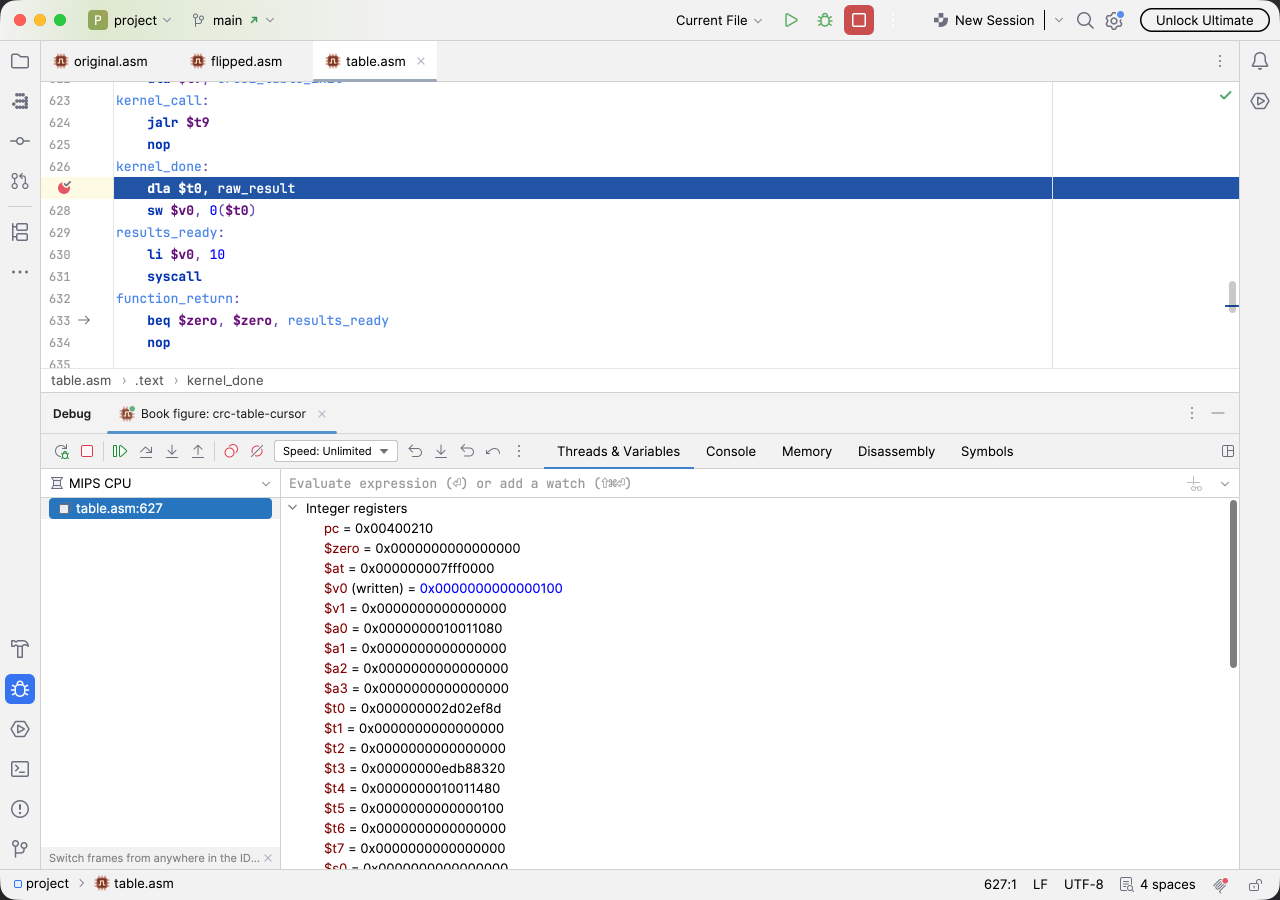
\includegraphics[width=0.50\linewidth,artifact,trim={\MARScrctablecursorLeft{} \MARScrctablecursorBottom{} \MARScrctablecursorRight{} \MARScrctablecursorTop{}},clip]{packages/024-crc32/captures/f02/cursor.png}};
\begin{scope}[shift={(cursor.south west)},x={($(cursor.south east)-(cursor.south west)$)},y={($(cursor.north west)-(cursor.south west)$)}]
\draw[black,line width=0.7pt] (0.023437500,0.023255814) rectangle (0.742187500,0.953488372);
\node[draw=black,fill=white,circle,inner sep=1.5pt,font=\footnotesize] at ($(0.023437500,0.953488372)+(-3mm,0)$) {3};
\end{scope}
\node[anchor=north west,inner sep=0,font=\small\bfseries] (zero-title) at ([yshift=-1mm]cursor.south west) {First table entries};
\node[anchor=north west,inner sep=0] (zero) at ([yshift=-1mm]zero-title.south west) {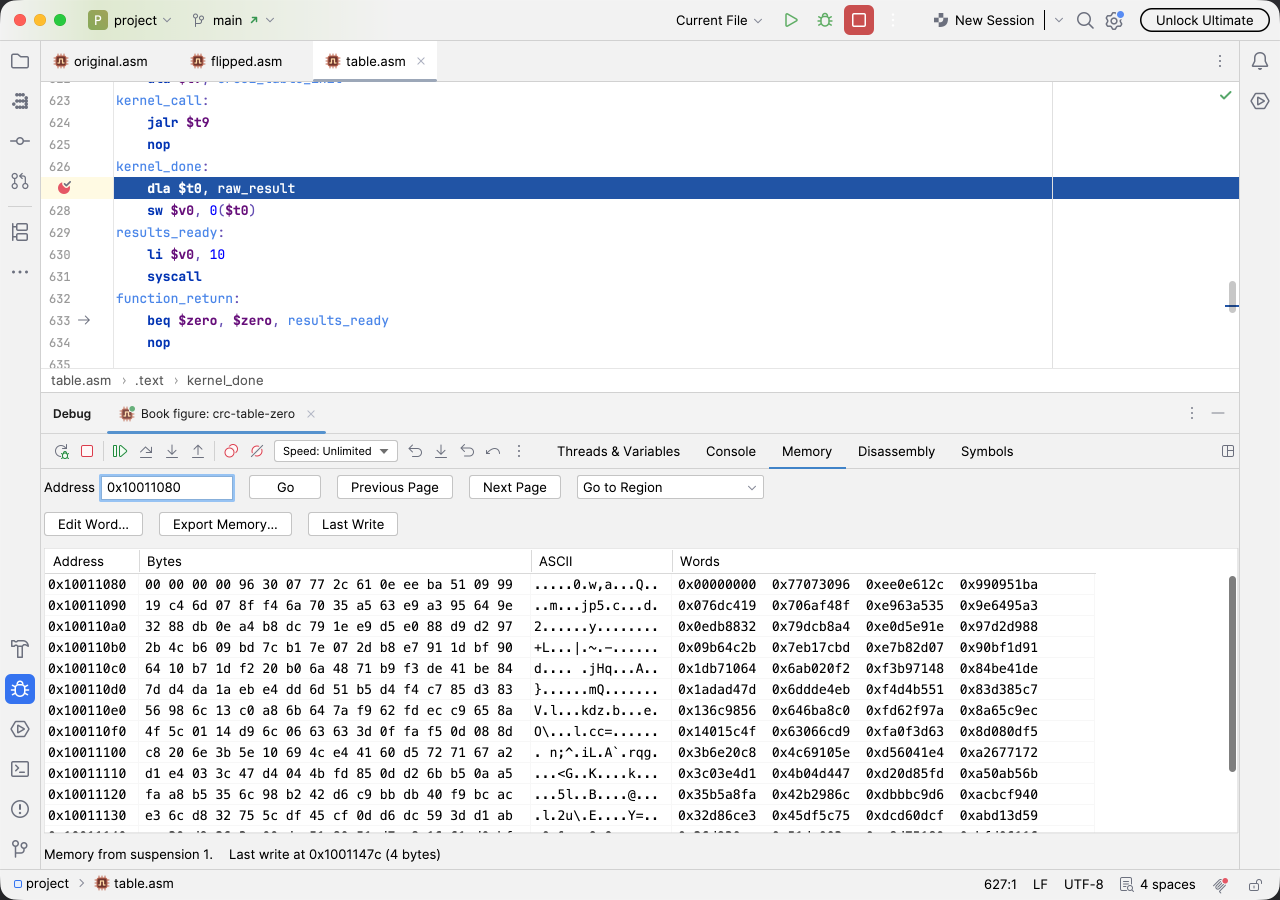
\includegraphics[width=0.84\linewidth,artifact,trim={\MARScrctablezeroLeft{} \MARScrctablezeroBottom{} \MARScrctablezeroRight{} \MARScrctablezeroTop{}},clip]{packages/024-crc32/captures/f02/zero.png}};
\begin{scope}[shift={(zero.south west)},x={($(zero.south east)-(zero.south west)$)},y={($(zero.north west)-(zero.south west)$)}]
\draw[black,line width=0.7pt] (0.194672131,0.078431373) rectangle (0.997950820,0.490196078);
\node[draw=black,fill=white,circle,inner sep=1.5pt,font=\footnotesize] at ($(0,0.490196078)+(-3mm,0)$) {4};
\end{scope}
\node[anchor=north west,inner sep=0,font=\small\bfseries] (middle-title) at ([yshift=-1mm]zero.south west) {Entry 128 and its neighbors};
\node[anchor=north west,inner sep=0] (middle) at ([yshift=-1mm]middle-title.south west) {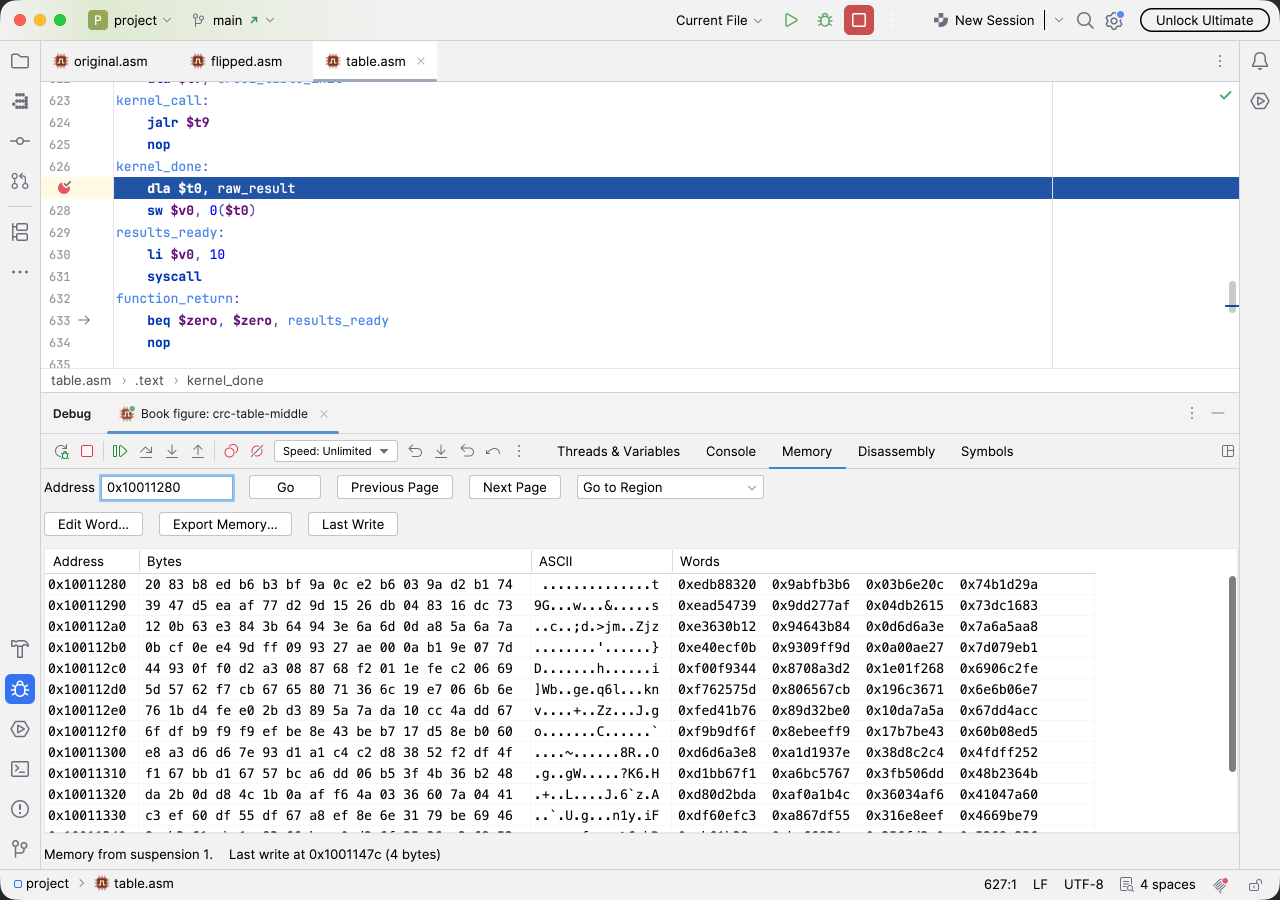
\includegraphics[width=0.84\linewidth,artifact,trim={\MARScrctablemiddleLeft{} \MARScrctablemiddleBottom{} \MARScrctablemiddleRight{} \MARScrctablemiddleTop{}},clip]{packages/024-crc32/captures/f02/middle.png}};
\begin{scope}[shift={(middle.south west)},x={($(middle.south east)-(middle.south west)$)},y={($(middle.north west)-(middle.south west)$)}]
\draw[black,line width=0.7pt] (0.194672131,0.078431373) rectangle (0.997950820,0.490196078);
\node[draw=black,fill=white,circle,inner sep=1.5pt,font=\footnotesize] at ($(0,0.490196078)+(-3mm,0)$) {5};
\end{scope}
\node[anchor=north west,inner sep=0,font=\small\bfseries] (tail-title) at ([yshift=-1mm]middle.south west) {Final entries and logical suffix};
\node[anchor=north west,inner sep=0] (tail) at ([yshift=-1mm]tail-title.south west) {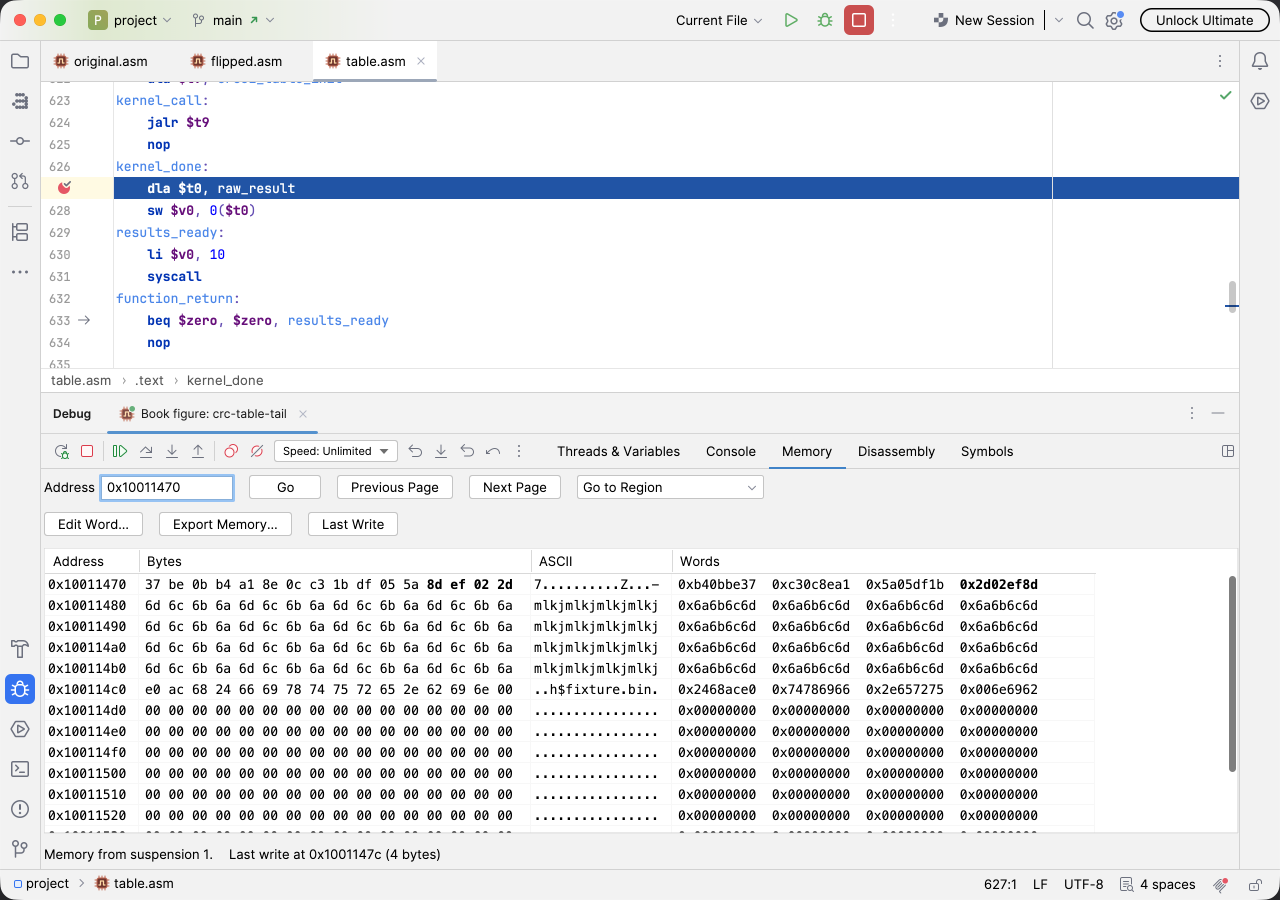
\includegraphics[width=0.84\linewidth,artifact,trim={\MARScrctabletailLeft{} \MARScrctabletailBottom{} \MARScrctabletailRight{} \MARScrctabletailTop{}},clip]{packages/024-crc32/captures/f02/tail.png}};
\begin{scope}[shift={(tail.south west)},x={($(tail.south east)-(tail.south west)$)},y={($(tail.north west)-(tail.south west)$)}]
\draw[black,line width=0.7pt] (0.194672131,0.055555556) rectangle (0.997950820,0.638888889);
\node[draw=black,fill=white,circle,inner sep=1.5pt,font=\footnotesize] at ($(0,0.638888889)+(-3mm,0)$) {6};
\end{scope}
\node[anchor=north west,inner sep=0,font=\small\bfseries] (guard-title) at ([yshift=-1mm]tail.south west) {Physical guard and following path bytes};
\node[anchor=north west,inner sep=0] (guard) at ([yshift=-1mm]guard-title.south west) {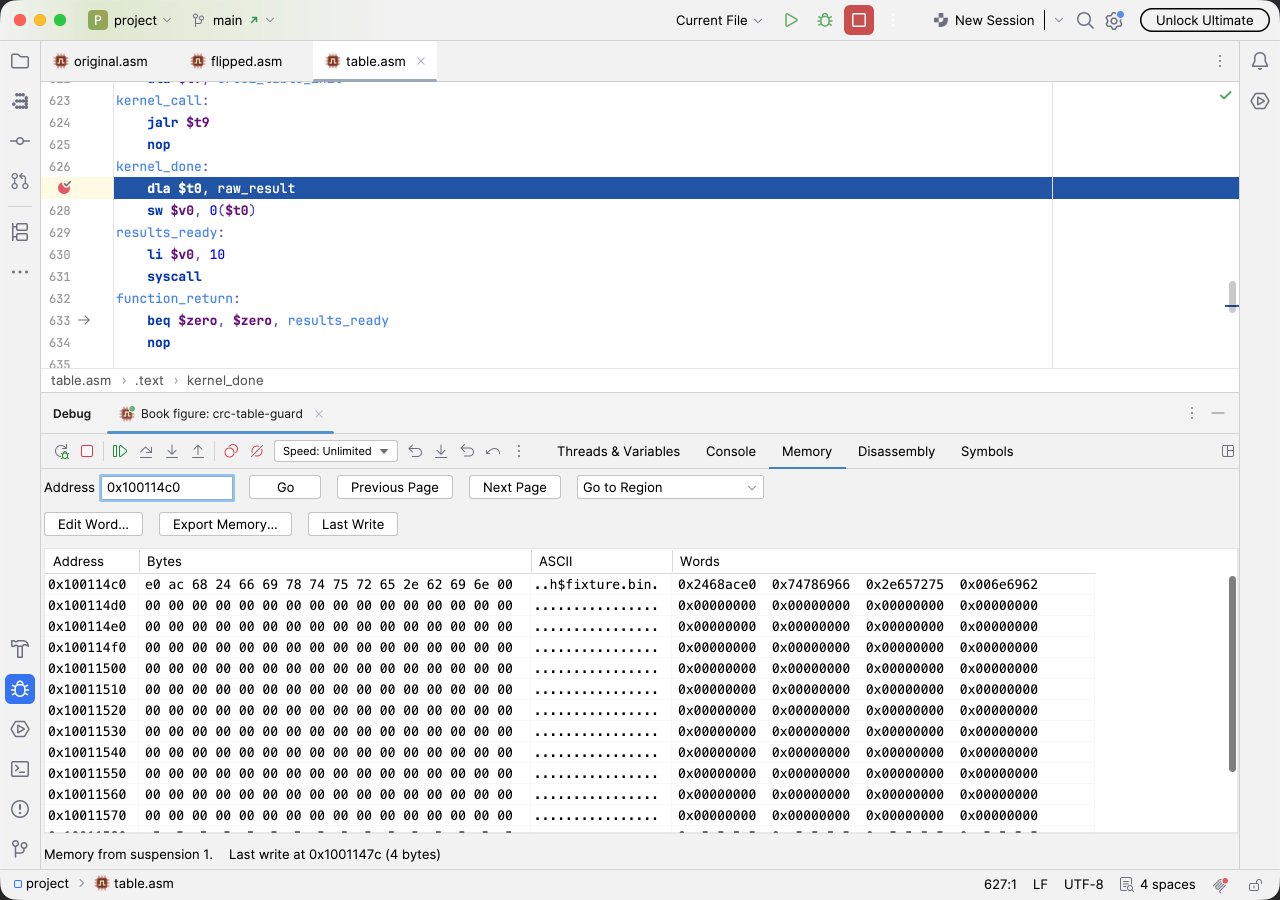
\includegraphics[width=0.84\linewidth,artifact,trim={\MARScrctableguardLeft{} \MARScrctableguardBottom{} \MARScrctableguardRight{} \MARScrctableguardTop{}},clip]{packages/024-crc32/captures/f02/guard.png}};
\begin{scope}[shift={(guard.south west)},x={($(guard.south east)-(guard.south west)$)},y={($(guard.north west)-(guard.south west)$)}]
\draw[black,line width=0.7pt] (0.194672131,0.078431373) rectangle (0.997950820,0.490196078);
\node[draw=black,fill=white,circle,inner sep=1.5pt,font=\footnotesize] at ($(0,0.490196078)+(-3mm,0)$) {7};
\end{scope}
\end{tikzpicture}
\par\smallskip
\begin{minipage}{\linewidth}
\small
\begin{enumerate}
\setlength{\itemsep}{0pt}
\setlength{\parsep}{0pt}
\item The stop at \texttt{kernel\_done} follows initialization and precedes the caller store. This return counts entries, rather than CRC state.
\item \texttt{v0 = 0x100} is the entry count 256. It counts words, so the logical table occupies 1024 bytes.
\item \texttt{t4 = 0x10011480} points immediately beyond those 256 words, and \texttt{t5 = 0x100} confirms the completed loop count. The table begins at \texttt{0x10011080}.
\item Entry zero is zero. The other words in this row are entries one through three; each is the raw zero-seeded result of processing its index byte.
\item Entry 128 at \texttt{0x10011280} is \texttt{edb88320}, stored low byte first as \texttt{20 83 b8 ed}. This is the reflected feedback mask.
\item The upper row contains entries 252 through 255. Its last word, entry 255, is \texttt{2d02ef8d} (\texttt{8d ef 02 2d}). The next row retains \texttt{0x6a6b6c6d} sentinels; these are backing storage beyond the logical table.
\item The physical guard at \texttt{0x100114c0} remains \texttt{2468ace0}. Following bytes belong to the path string, not another table entry.
\end{enumerate}
\end{minipage}
\caption{The initializer writes all 256 entries while leaving the logical suffix and guard untouched.}
\label{capture:024-crc32-f02}
\label{crc-f02}
\end{figure}
\par
